% Preamble {{{
% Fixs the conflict of hyperref with moderncv class
\PassOptionsToPackage{unicode}{hyperref}

\documentclass[11pt,a4paper,sans]{moderncv}
\usepackage{etoolbox}

% Moderncv themes
% ----------------------------------------
\moderncvstyle{banking} % 'casual', 'classic', 'oldstyle' and 'banking'
\moderncvcolor{blue} % 'blue', 'orange', 'green', 'red', 'purple', 'grey' and 'black'

% '\sfdefault' for the default sans serif font
% '\rmdefault' for the default roman one, or any tex font name
%\renewcommand{\familydefault}{\sfdefault}
%\nopagenumbers{}

\usepackage[T1]{fontenc} % Character encoding
%\usepackage{lmodern}
%\usepackage{charter}
% \usepackage[bitstream-charter]{mathdesign} % Font
\usepackage[ngerman]{babel} % Neu deutsche Rechtschreibung
\usepackage[utf8]{inputenc} % UTF-8 encoding
\usepackage{bookmark}

% adjust the page margins
%\usepackage[scale=0.75]{geometry}
\usepackage[left=2cm, right=2cm, top=2cm, bottom=2cm]{geometry}
\setlength{\hintscolumnwidth}{3.5cm} % Width of the column with the dates
%\setlength{\makecvtitlenamewidth}{10cm} % Width allocated to your name

% personal data
\firstname{Ngoc Minh}
\familyname{Dao}
\title{Lebenslauf}
\address{Bömelburgstr. 18B}{30165 Hannover}{Deutschland}
\phone[mobile]{+49 17674561589}
\email{ngocminhdao88@gmail.com}
%\phone[fixed]{+2~(345)~678~901}
%\phone[fax]{+3~(456)~789~012}
%\homepage{www.johndoe.com}
\social[linkedin]{ngocminhdao}
\social[xing]{NgocMinh\_Dao}
%\social[github]{jdoe}
\extrainfo{Geboren am 24.03.1988 in Hai Duong, Viet Nam}
%\extrainfo{}
%\photo[85pt][0.4pt]{./bilde/NgocMinhDao-Bewerbungsfoto.jpg}
%\quote{Some quote}

%\makeatletter % to show numerical labels in the bibliography
%\renewcommand*{\bibliographyitemlabel}{\@biblabel{\arabic{enumiv}}}
%\makeatother
%\renewcommand*{\bibliographyitemlabel}{[\arabic{enumiv}]}

% bibliography with mutiple entries
%\usepackage{multibib}
%\newcites{book,misc}{{Books},{Others}}% }}}

% custom footer on the other pages
\fancyfoot[RE,LO]{\parbox[b]{15cm}{\color{color2}\addressfont\strut Ngoc Minh Dao~~\emailsymbol\emaillink{ngocminhdao88@gmail.com}~~\faMobile~{+49 17674561589} \\ ~~\httplink[\faLinkedin~ngocminhdao]{linkedin.com/in/ngocminhdao}~~\httplink[\faXingSquare~ngocminhdao]{xing.com/profile/NgocMinh_Dao}}}
\rfoot{}

% macros
\newcommand {\myFirstName} {Ngoc Minh}
\newcommand {\myLastName} {Dao}

\begin{document}
% ----------------------------------------
% Lebenslauf
% ----------------------------------------

% create a new bookmark for Lebenslauf
\bookmark[page=\thepage, level=-2]{Lebenslauf von Ngoc Minh Dao}
\thispagestyle{empty}
\hskip -3.5cm {\makecvtitle} % Lebenslauf Title

% Bewerbungsfoto
\begin{picture}(0,0)
    \put(380, 0){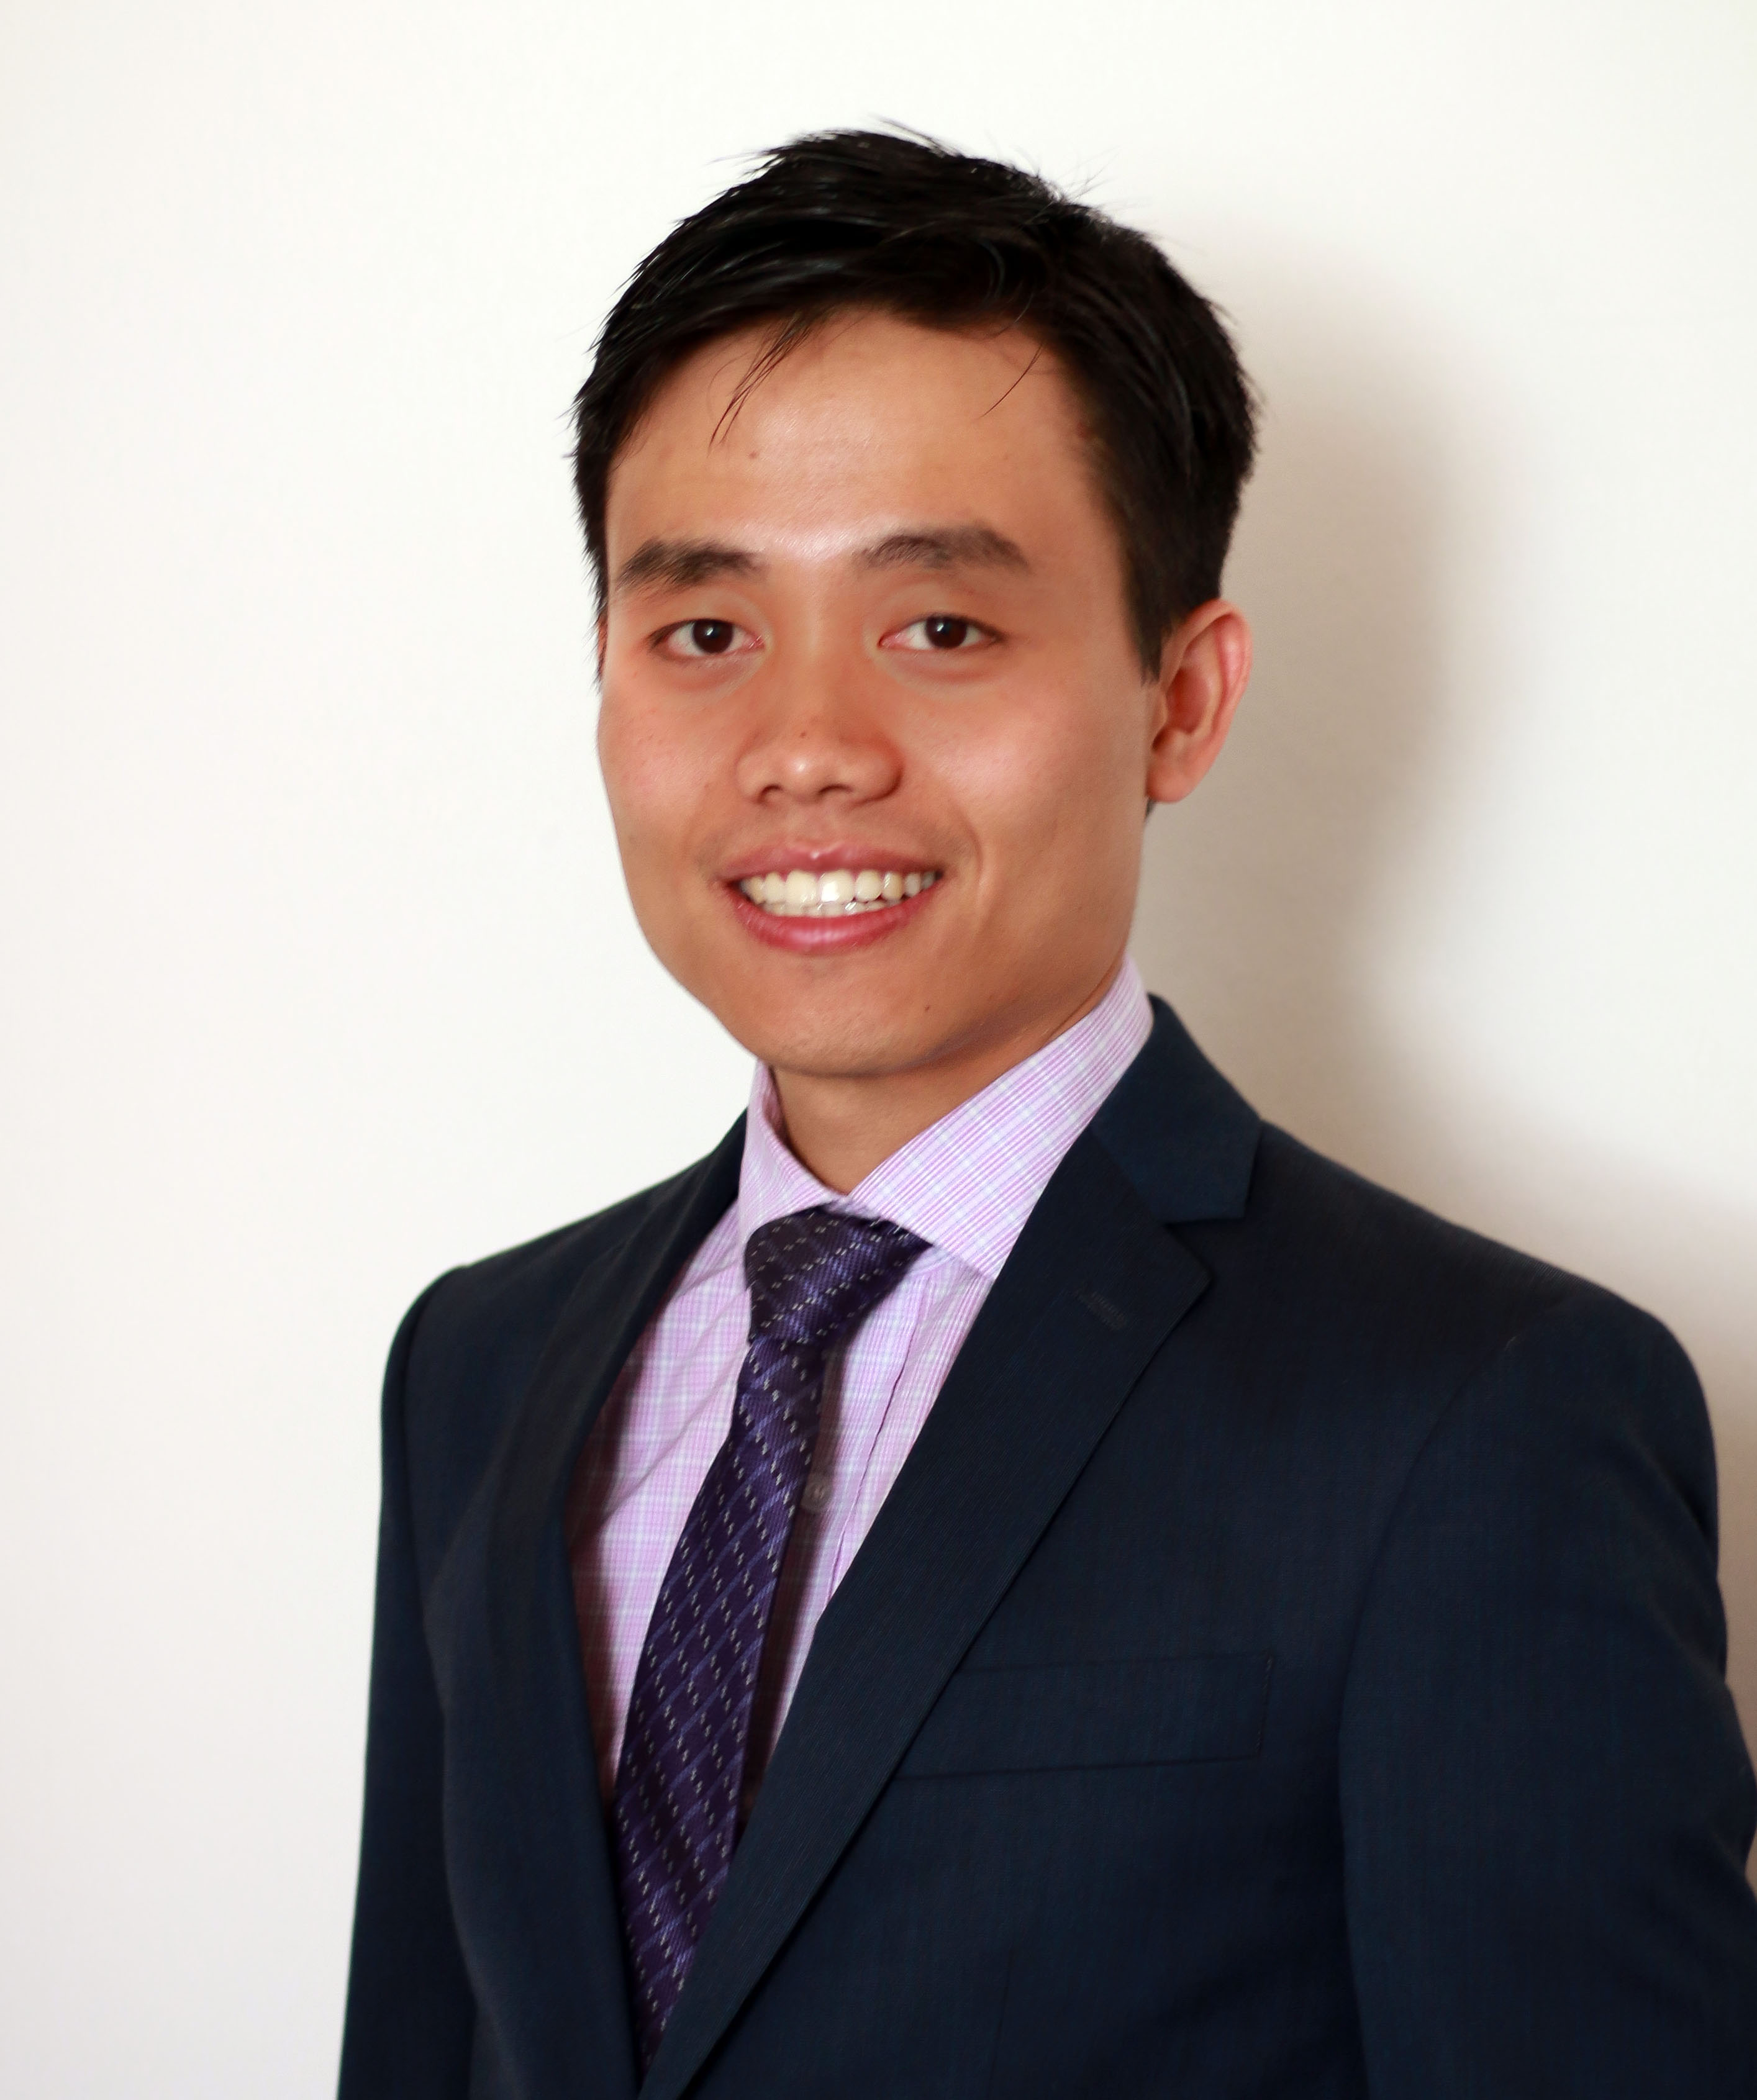
\includegraphics[scale=0.15]{./bilde/NgocMinhDao_Bewerbungsfoto.jpg}}
\end{picture}

% Praktika {{{
\section{\textbf{Praktika}}
% Praktikum bei Schaeffler Gruppe
\cventry{03.2017--09.2017}
{Praktikum im Bereich Anwendungstechnik}
{Schaeffler Technologies AG \& Co. KG}
{Herzogenaurach, Deutschland}
{}
{
    \begin{itemize}
        \item Berechnung von Fahrzeuggetrieben
        \item Untersuchungen an Lagern aus Feldausfällen
        \item Benchmarkuntersuchungen an Kugellagern verschiedener Wettbewerber
        \item Empfang und Büromanagement sowie Unterstützung der Geschäftsleitung
    \end{itemize}
}
%}}}


% Berufserfahrung {{{
\section{\textbf{Berufserfahrung}}

% Hiwijob bei IMKT - Giovanno Moebes
\cventry{10.2015--02.2017}
{Institut für Maschinenkonstruktion und Tribologie}
{Wissenschaftliche Hilfskraft}
{Hannover, Deutschland}
{}
{
Montage und Demontage von Prüfständen.
Programmierung und Aufbau von Prüfstandsteuerungen zur Wälzlager-Untersuchungen.
Analyse und Auswertung der Messreihen.
}

% Hiwijob bei Micreon GmbH - Frank Korte
\cventry{09.2015--02.2017}
{Micreon GmbH}
{Werkstudent}
{Hannover, Deutschland}
{}
{
Programmierung einer Überwachungsoftware zum Aufnehmen des Arbeitsdrucks der Laser-Schneide-Maschinen.
Aufbau von elektronischen Laborinstrumenten.
Qualitätsinspektion der lasergeschnitten Teilen.
}

%% Hiwijob bei IFW - Maik Bergmeier
%\cventry{09.2015--03.2016}
%{Institut für Fertigungstechnik und Werkzeugmaschinen}
%{Wissenschaftliche Hilfskraft}
%{Garbsen, Deutschland}
%{}
%{
%Analyse, Auswertung und Präsentation von Messdaten eines Schraubenherstellung-Projekts.
%}
%}}}


% Ausbilung {{{
\section{\textbf{Ausbildung}}

% Master
\cventry{10. 2009 -- 06.2018}
{Master of Science, Maschinenbau (Konstruktion, Fahrzeugsysteme)}
{Leibniz Universität Hannover}
{Hannover, Deutschland}
{}
{
    Masterarbeit:
    \begin{itemize}
        \item ``Entwicklung eines modularen Messsystems zur optischen und kapazitiven Schmierfilmdickenmessung in einem EHD-Kontakt''
    \end{itemize}
    %
    Projektarbeit:
    \begin{itemize}
        \item "`Ausarbeitung eines Prüfkonzeptes zur Untersuchung der Dichtwirkung von Radialwellendichtringe unter Fliehkrafteinfluss"'
    \end{itemize}
}

% Bachelor
\cventry{09.2006--06.2009}
{Bachelor of Science, Maschinenbau (Konstruktion)}
{Hanoi University of Science and Technology}
{Ha Noi, Viet Nam}
{}
{
    Bachelorarbeit:
    \begin{itemize}
        \item "`Konstruktion und Fertigung von Werkzeughaltern und deren speziellen Einsätze"'
        %\item Betreuer: Dr.-Ing. Duy Liem Ta
        %\item Note: 8.5/10
    \end{itemize}
}

%% Highschool life
%\cventry{09.2003--06.2006}
%{Abitur}
%{Minh Tan Oberschule}
%{Hai Duong, Viet Nam}
%{}
%{}
%}}}


% Weiterbildung, Kurse und Seminare {{{
\section{\textbf{Weiterbildungen, Kurse und Seminare}}

% A Hands-on Introduction to Engineering Simulations - CornellX
\cventry{05.2018--vsl. 08.2018}
{Finite-Elemente-Analyse und numerische Strömungsmechanik mit ANSYS}
{A Hands-on Introduction to Engineering Simulations}
{CornellX}
{}
{}


% Introduction to Project Management - AdelaideX
\cventry{06.2018--vsl. 08.2018}
{Initialisierung, Planung, Ausführung etc. von Arbeiten}
{Introduction to Project Management}
{AdelaideX}
{}
{}


% Automatikgetriebe Schulung
\cventry{07.2017}
{
    \parbox[t]{10cm}{Allgemeiner Überblick von Fahrzeuggetrieben und Vertiefung durch Beispiele aus Praxis}
}
{Automatikgetriebe Schulung}
{Schaeffler Technologies AG \& Co. KG}
{}
{}


% Multisoft Virtual Academy - Creo
\cventry{11.2016}
{Von digitalen Ideen bis zur Herstellung von Produkten}
{PTC Creo Training}
{Multisoft Virtual Academy}
{}
{}

%% LabVIEW - CLAD Prüfung
%\cventry{10.2016}
%{}
%{Certified LabVIEW Associate Developer}
%{National Instrument}
%{}
%{}


% Autodesk Inventor Professional Workshop
\cventry{7.2016}
{Dreitätiges Instructor-led-Training mit verschiedenen Themen und Modellierungstechniken}
{Autodesk Inventor Professional Workshop}
{ITA - LUH}
{}
{}


%% Online course on edx mooc - Programming with C#
%\cventry{02.2016--04.2016}
%{Programming with C\# (DEV204x)}
%{Microsoft}
%{edX Inc}
%{}
%{
%    \begin{itemize}
%        \item Online Kurs: 8 Wochen mit je 8-10 Wochenstunden
%    \end{itemize}
%}

%% Online course on edx mooc - Embedded Systems - Shape the World
%\cventry{01.2016--04.2016}
%{Embedded Systems - Shape the World (UT.6.03x)}
%{UTAustinX}
%{edX Inc}
%{}
%{
%    \begin{itemize}
%        \item Online Kurs: 12 Wochen mit je 8 Wochenstunden
%    \end{itemize}
%}

% Online course on edx mooc - Introduction to computer science and programming using python
\cventry{01.2016}
{Rechnerische und algorithmische Denkweise zur Problemlösung}
{Introduction to Computer Science and Programming using Python}
{MITx}
{}
{}

%% Online course on edx mooc - Introduction to python for data science
%\cventry{01.2016--02.2016}
%{Introduction to Python for Data Science (DAT208x)}
%{Microsoft}
%{edX Inc}
%{}
%{
%    \begin{itemize}
%        \item Online Kurs: 4 Wochen mit je 4 Wochenstunden
%    \end{itemize}
%}

%% Fernlerngang beim Christiani Akademie - CAD-Kompakt
%\cventry{11.2015--04.2016}{CAD-Kompakt mit Solidworks}
%{Christiani Akademie}{Konstanz, Deutschland}{}{
%  \begin{itemize}
%    \item Fernlerngang: 6 Monaten mit je 5 Wochenstunden
%  \end{itemize}
%}
%}}}

% EDV-Kenntnisse {{{
\section{\textbf{EDV-Kenntnisse}}

% CAD/CAE
\cvitem{CAD/CAE}{Gute Kenntnisse in Creo, Inventor, Solidworks und ANSYS}

% Programming
\cvitem{Programmiersprache}{Gute Kenntnisse in LabVIEW, \texttt{C/C++}, Python und Matlab}

% Software
\cvitem{Textverarbeitung}{\LaTeX~und MS Office}

\cvitem{Bildverarbeitung}{CorelDRAW und GIMP}

%}}}

% Engagement und Hobbys {{{
\section{\textbf{Engagement und Hobbys}}

% Schaeffler Sportbetrieb
\cventry{03.2017--09.2017}
{
Laufen mit Schaeffler-Arbeitskollegen
}
{Lauftreff}
{Herzogenaurach, Deutschland}
{}
{}

% Arduino Hannover
\cventry{10.2016--02.2017}
{
Treffen und Diskutieren über elektronische Projekte
}
{Arduino Hannover}
{Hannover, Deutschland}
{}
{}

% AKAKRAFT Mitglied
\cventry{03.2015--05.2015}
{
\parbox[t]{12cm}{KFZ Inspektion, Ölwechsel, Zerlegung und Montage von Motoren und Getrieben}
}
{Akademische Gruppe für Kraftfahrwesen (AKAKRAFT)}
{Hannover, Deutschland}
{}
{}

% Badminton sport
\cventry{seit 2013}
{
\parbox[t]{10cm}{Mannschaftsmitglied in der 1.Kreisliga des niedersächsischen Badminton-Verbands}
}
{Badminton}
{Hannover, Deutschland}
{}
{}
%}}}

% Spachen {{{
\section{\textbf{Sprachen}}
\cvitemwithcomment{Englisch}{Gute Kenntnisse}{}
\cvitemwithcomment{Deutsch}{Gute Kenntnisse}{}
\cvitemwithcomment{Vietnamesisch}{Fließend}{Muttersprache}
% }}}

% Qualifikation {{{
\section{\textbf{Qualifikation}}
\cvitem{Führerschein}{PKW Klasse B}
\cvitem{National Instrument}{LabVIEW Certified Associate Developer}
%}}}

\end{document}
